\documentclass[10pt]{amsart}
\usepackage{amsmath,amsfonts,amssymb,amsthm,epsfig,color,tikz,hyperref,tkz-euclide}

\begin{document}

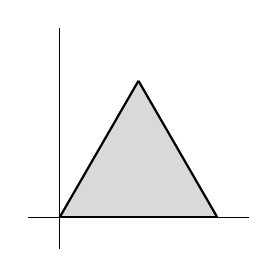
\begin{tikzpicture}[scale=2.0]

% Draw coordinate axes (background)
\draw(-0.2,0) -- (1.2,0);
\draw(0,-0.2) -- (0,1.2);

% Fill the triangle (60-degree angle at origin, unit sides)
\fill[gray!30] (0,0) -- (1,0) -- (60:1) -- cycle;

% Draw triangle edges
\draw[thick] (0,0) -- (1, 0);
\draw[thick] (0,0) -- (60:1);
\draw[thick] (1,0) -- (60:1);

\end{tikzpicture}

\end{document}